\chapter{Entwicklung einer real-time Query Anwendung zur Beschleunigung von Userprofilqueries}
Ein wesentlicher Bestandteil der bestehenden Betriebsanwendung bildet das Abfragen von Userprofildaten. Um für Umfragen passgenau Teilnehmer auszuwählen, gibt es in der Profildatenbank, die knapp 400.000 Nutzer umfasst, 176 Profilfelder. Diese können in allen denkbaren Kombinationen abgefragt werden. Die besteheden Datenbankabfragen geschehen aufgrund ihrer langen Laufzeit asynchron. Hier soll eine neue, synchrone Schnittstelle geschaffen werden.

\section{Real-time Anforderungen erzwingen eine neue Entwicklung}
Da das Finden von Umfrageteilnehmern und demnach das Abfragen der Profilfelder einen wesentlichen Kern der Betriebsanwendung bildet, besteht dieser Teil der Anwendung mit am längsten. In den fast 3 1/2 Jahren ist sowohl die Anzahl der User, also auch die Anzahl der Profilfelder enorm gewachsen, weitaus mehr als initial erwartet. Im Laufe der Zeit stellte sich heraus, das die gewählte Datenbanktechnologie MongoDB, die gewählte Datenstruktur und die Art wie gequeried wird, nicht optimal und daher nicht schnell genug sind. Da das Abfragen der Profilfelder wesentlichster Bestandteil des Kerngeschäfts ist und die Defizite die Situation mit wachsender User- und Kundenzahl nur verschärfen, wurde deutlich, dass eine Überarbeitung der bestehenden Strukturen notwendig ist.

Das Ziel der Neuentwicklung ist vor Allem, die Queries zu beschleunigen. Da viele Queries, besonders auf solche Felder, die nicht durch einen Index abgedeckt sind, sehr langsam sind, soll hier eine signifikante Zeitersparnis erreicht werden. Zum Anderen soll aber gleichzeitig auch die Struktur des Codes verbessert werden. Fast die gesamte Anwendung befindet sich zur Zeit in einem Repository. Die Strukturen sind zum Teil sehr vermischt und Abhänigkeiten bestehen auch dort, wo keine bestehen sollten. Der neu entworfene Code soll klare Strukturen und klare Schnittstellen besitzen.

\section{Majestic Monolith vs Minimal Microservice}
Um die genannten Probleme zu lösen muss zunächst eine Analyse der Ausgangssituation durchgeführt werden. Es können jedoch grundsätzlich verschiedene Lösungsansätze zur Optimiertung verfolgt werden. Zum Einen kann eine neue Datenbanktechnologie mit optimiertem Schema gewählt werden. Zum Anderen kann der Code kann auf Geschwindigkeit optimiert oder komplett neu geschrieben werden.
Da die in der Anwendung eingesetzte Datenbank MongoDB noch für weitere Teile der Anwendung genutzt wird, kann sie nicht komplett ausgetauscht werden. Da es sich jedoch zur Optimierung sowohl anbietet eine neue Datenbanktechnologie einzusetzen, als auch den Code zu verbessern, bietet sich die Entwicklung eines separaten Microservices an. Hier kann eine optimierte Datenbanktechnologie eingesetzt werden ohne die bestehende Anwendung um weitere Strukturen zu ergänzen. Weiterhin kann der Code komplett restrukturiert und Komplexität verschoben werden. Der bestehende Code kann komplett ersetzt werden und somit kann die Struktur verbessert werden.
Des Weiteren erlaubt es ein separater Service, passgenauere Skalierung. Durch dynamisches Hosting kann so also nicht nur die inhärente Performance von Code und Datenbank verbessert werden, sondern die reale auch dadurch, Ressourcen optimiert einzusetzen.
Da eine neue Datenbanktechnologie und ein komplett separater Service ohnehin mit vielen Änderungen verbunden ist, wurde beschlossen den alten Code nicht in einen neuen Service zu migrieren, sondern die Funktionalität neu zu Schaffen.

\section{Mit dem Strangler Pattern vom Monolithen zur Microservice Architektur}
Da die aktuelle Arbeitslage, die vorhandenen Entwickler und die Größe der Anwendung es nicht zulassen diese direkt komplett zu überarbeiten, wird hier die Architektur mit Hilfe des Strangler Patterns~\footcite[][]{Fowler:Strangler} Schritt für Schritt umgesetzt.
Der Name des Stangler Patterns ist aus einer Analogie zur Botanik entstanden. Hierbei wurde von Fowler der Vergleich zur Würgefeige (engl. Strangler Fig) gezogen. Diese wächst von den Ästen an einem Wirtsbaum herab, bis sie den Boden erreicht. Nach und nach wird der Wirtsbaum immer weiter umschlossen, bis er schließlich abstirbt.
Ähnlich kann bei der Softwareentwicklung zum Ersetzen einer alten Anwendung vorgegangen werden. An bestimmten, sich eignenden Stellen wird begonnen Teile der bestehenden Anwendung zu ersetzen. Neuer Code wird geschaffen und nach und nach die Last auf die neue Teilanwendung geleitet.
Dieses Vorgehen bietet viele Vorteile gegenüber dem kompletten Austausch einer Altanwendung. Die neue Anwendung kann Stück für Stück mit agilen Methoden und häufigen deploys entwickelt und im Produktionsbetrieb betrachtet werden. Die neu entstehende Anwendung kann hierbei nach Belieben angepasst werden, um die Altanwendung am problemlosesten zu Ersetzen.
Zur Umsetzung dieses Ersetzens gibt es viele Wege. Zwei ebenfalls von Fowler vorgebrachte Strategien sind AssesCapture~\footcite[][]{Fowler:Capture} und EventInterception~\footcite[][]{Fowler:Interception}.
Beim AssetCapture geht es vor Allem darum, Assets zu identifizieren, die sich leicht in die neue Teilanwendung migrieren lassen. Dies können bestimmte Tabellen in der Datenbank sein. Im Fall der zu entwickelnden Anwendung sind dies die Userprofile.
EventInterception geht mit AssetCapture Hand in Hand. Hierbei müssen alle Events auf die ausgelagerten Assets, also zum Beispiel das Abfragen von Profilen und das Anlegen neuer Profile, abgefangen und umgeleitet werden.
So wird sichergestellt, dass die alten Ressourcen nicht mehr aktualisiert werden und es nicht zu Inkonsitenzen im Datenbestand kommt.
Um die bestehende Betriebsanwendung auf Microservices umzustellen, wird hier ähnlich vorgegangen. Aus gegebenem Anlass wird der Query-Microservice als erster Strangler entwickelt. Die Userprofile eignen sich gut um sie in eine neue Datenbank zu migrieren und in diesem Schritt gleich zu optimieren. Ein neuer Service verwaltet hierzu den Zugriff auf die Daten. Die bestehenden Events zum Abfragen von Userprofildaten werden auf den neuen Service umgestellt. Hier wird eine Schnittstelle geschaffen, die sowohl Zugriff auf den neuen Service, als auch auf die alte Datenbank zulässt. Wird eine neue Anwendung mit Userschnittstelle geschaffen, bietet es sich an einfach nach und nach mehr der Seitenzugriffe auf das neue System umzuleiten. Zum Einen auf Makroebene, also Feature für Feature ablösen, aber auch auf Mikroebene bei ersetzen eines Features. So können Fehler im neuen System minimiert werden und die Belastbarkeit des Systems sichergestelllt werden.
\begin{figure}[h]
    \caption{Load Balancer zur Strangulation Verteilung (\cite{Hammant:Strangler})}
    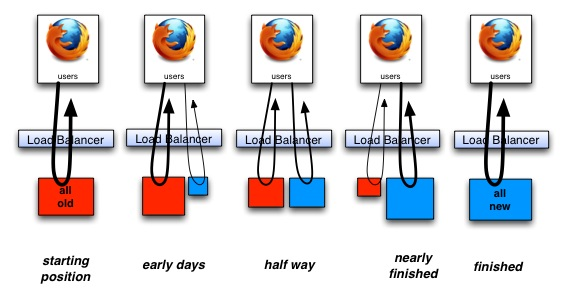
\includegraphics[width=\textwidth]{strangulation}
\end{figure}

Da der entwicklete Microservice keine Schnittstelle zum Web, sondern nur zum bereits bestehenden Monolithen hat, beschloss ich hier statt mit einem Load Balancer, mit Hilfe des Ruby Flipper Gems\footnote{https://github.com/jnunemaker/flipper} nach und nach mehr Last auf den neu entstehenden Service zu verteilen.~\footcite[vgl.][]{Hammant:Strangler} So kann beispielsweise für bestimmte Nutzer der neue Dienst aktiviert werden, während alle anderen Nutzer noch den alten Service nutzen können. Dies dient zum Einen dem Testen des neuen Services auf Fehler, sowie auch zur Evaluierung dessen Performance.
Hierzu wird die zentrale Schnittstelle des QueryExecuters geschaffen. Die bestehende Struktur, Mongoid, wird abstrahiert und um eine weitere für die neue API, den Propheten, ergänzt. Diese von den beiden Klassen gebotenen Schnittsellen sind identisch. Der QueryExecuter verteilt lediglich anhand der Flipper Logik an den neuen Microservice oder den bestehenden Code.

Da die Userprofile noch auf Seiten der Verwaltung der User selbst in der Hauptanwendung benötigt werden, werden hier jedoch nicht alle Events abgefangen. Lediglich die, die das Querien im Bereich des Samplings betreffen. Um Datenkonsitenz zu gewährleisten, werden einmal täglich alle veränderten Daten in den Microservice geupdated. Da sich Userdaten nicht häufig ändern und sich unter 100 Nutzer am Tag registrieren, reicht dies aus um ausreichend gute Query Ergebnisse zu erzielen.